\subsection{The simulation of PID}

\begin{figure}[H]
    \begin{center}
    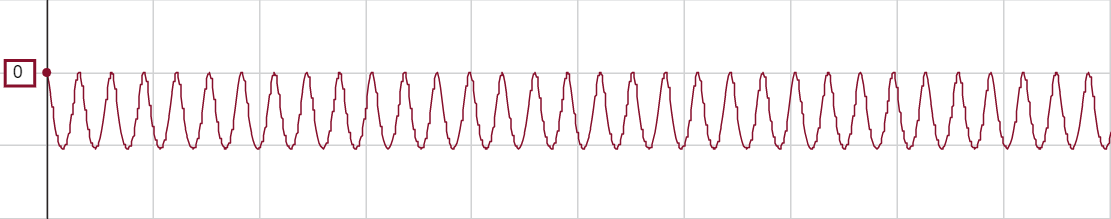
\includegraphics[scale=0.75]{pictures/control/posc}
    \end{center}
    \caption{Example of a system tuned using the Ziegler-Nichols method\cite{LibrePID}}
    \label{fig:posc}
\end{figure}

\begin{figure}[H]
    \begin{center}
    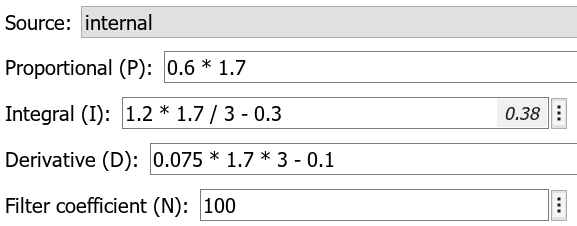
\includegraphics[scale=0.7]{pictures/control/simpidvalues}
    \end{center}
    \caption{Example of a system tuned using the Ziegler-Nichols method\cite{LibrePID}}
    \label{fig:simpidvalues}
\end{figure}

\begin{figure}[H]
    \begin{center}
    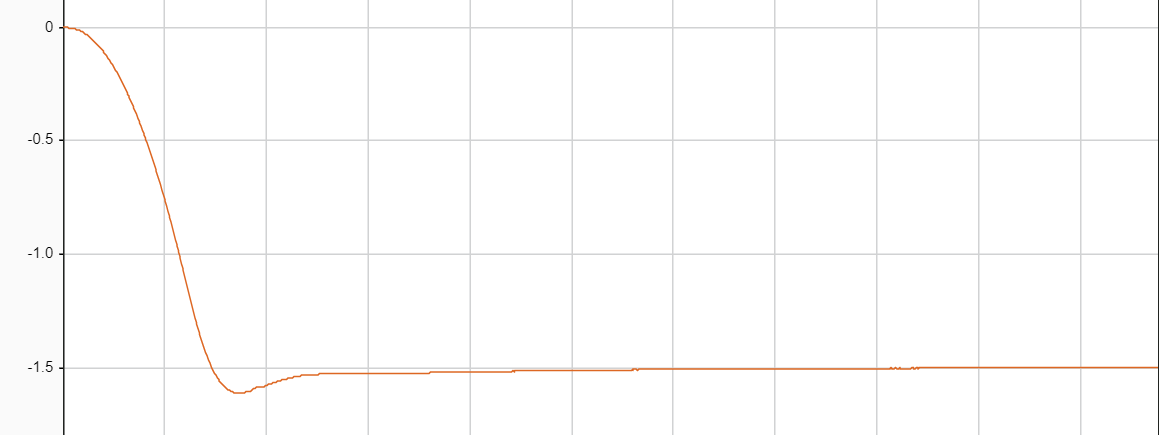
\includegraphics[scale=0.7]{pictures/control/zpidnonoise}
    \end{center}
    \caption{Example of a system tuned using the Ziegler-Nichols method\cite{LibrePID}}
    \label{fig:zpidnonoise}
\end{figure}

\begin{figure}[H]
    \begin{center}
    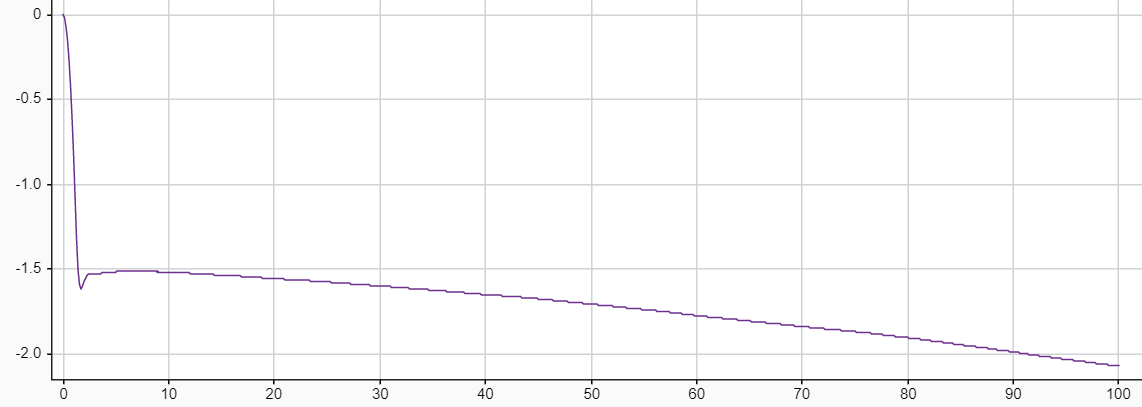
\includegraphics[scale=1]{pictures/control/zpidnoise}
    \end{center}
    \caption{Example of a system tuned using the Ziegler-Nichols method\cite{LibrePID}}
    \label{fig:zpidnoise}
\end{figure}
